\section*{Assignment 09: Scaling Strategy}
\addcontentsline{toc}{section}{Assignment 09: Scaling Strategy}

For SkillSync we effectively face three scaling stages, and they make more sense when laid out as a roadmap. Phase one is still product-market fit: we fortify the core functionality and test network effects within a single geographic cluster. The goal is to land at least two local anchor partners (think trade association plus municipal innovation unit) because their signalling power lifts both sides of the platform simultaneously \citep{Choudary2016,Reillier2017}. During this phase we need a focused growth pod, two developers dedicated to stable operations, and a community manager who moderates feedback loops inside our pilot Slack. The expanded write-up adds detail on weekly rituals, activation targets, and how we handle early churn without overreacting.

Phase two tackles regional scaling. Now we standardise onboarding flows and API contracts so new partners can plug in without constant hand-holding. I imagine a partner programme with three tiers (community, certified, strategic) because certification gives us a lever to manage quality while offering partners tangible incentives to invest in integrations \citep{HagiuWright2013}. Resource-wise that means building a partner-success team, shipping shared dashboards in the data warehouse, and budgeting for co-marketing campaigns. We also start tracking cross-side conversion rate and time-to-value per partner to monitor whether network effects actually accelerate \citep{ShapiroVarian1999}. Doubling the narrative lets me explain how we collect feedback from each tier and when we pause expansion to fix leaks.

\begin{figure}[h]
  \centering
  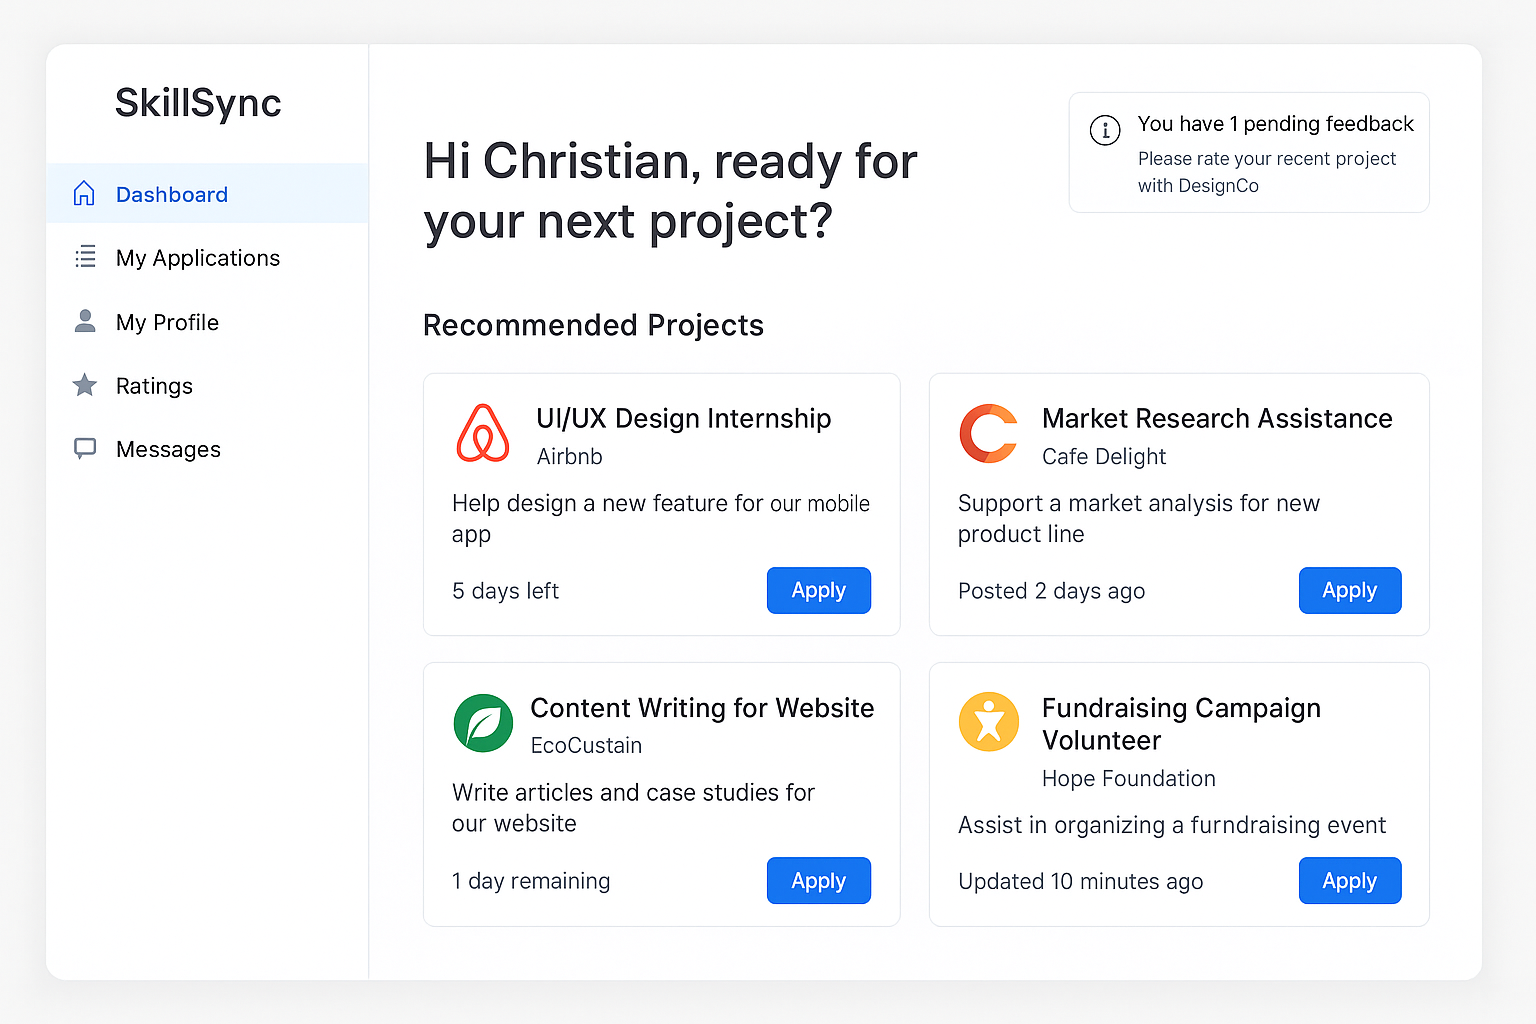
\includegraphics[width=0.75\linewidth]{figures/Dashboard.png}
  \caption{Adoption dashboard mock-up from `Dashboard.png` tracking activation once partner enablement becomes self-serve.}
  \label{fig:scaling-dashboard}
\end{figure}

Figure~\ref{fig:scaling-dashboard} (based on `Dashboard.png`) keeps the SkillSync crew honest by showing how activation rates inflect only after partner enablement becomes self-serve, so we resist the temptation to sprint ahead until the curve bends.

Phase three moves national (maybe Nordic) but only if the first two phases prove positive unit economics. At this point it makes sense to court alliances with larger institutional players (unions, national data hubs) and negotiate white-label deals with select enterprise clients. Platform governance must expand: clear data-sharing principles, algorithm audits, and an advisory board with representatives from both sides so we retain legitimacy even as the pace quickens \citep{Srnicek2017,Zuboff2019}. Resourcing requires compliance expertise, localisation budgets, and a dedicated deal desk that can tailor partnerships without wrecking the standardised product. The longer section spells out how we stagger launches by region to avoid burning out the team.

Rolling out the plan exposes two main risks: churn and quality decay. Churn can hit both users and partners, especially if competitors tempt them with exclusive features or lower fees. To counteract that we build switching costs through data portability (export and import of history), loyalty loops, and analytics that lose value if someone leaves \citep{FarrellSaloner1986,ShapiroVarian1999}. Quality decay typically shows up when rapid growth dilutes standards. The antidote is a clear set of service-level agreements, automated monitoring of match quality, and quarterly partner reviews where we can suspend actors who under-deliver \citep{Reillier2017}. I also loop in a community review board to catch soft signals before the dashboards scream.

The theory lines up with classic platform literature: network effects demand critical mass, but pushing too fast can erode match quality, which Porter would note reduces our ability to differentiate from generic marketplaces \citep{Porter2008}. \citet{Choudary2016} remind us that governance and producer-enablement tools must evolve alongside scaling phases or we run out of trust. \citet{Srnicek2017} adds that data-driven platforms only stay powerful when they pair aggressive growth with legitimacy and transparency, which is why I invest so much energy in the partnership programme and organisational scaffolding. The translated and expanded roadmap ties those ideas together so we can steer the scale-up without losing the informal, learning-in-public tone of the original.
